
\chapter{Opencv}

\section{Introduction }
OpenCV (Open Source Computer Vision Library) is released under a BSD license and hence it’s free for both academic and commercial use. It has C++, C, Python and Java interfaces and supports Windows, Linux, Mac OS, iOS and Android. OpenCV was designed for computational efficiency and with a strong focus on real-time applications. Written in optimized C/C++, the library can take advantage of multi-core processing. Enabled with OpenCL, it can take advantage of the hardware acceleration of the underlying heterogeneous compute platform. 
\subsection{Build and install Opencv with Opencv Contrib}

\begin{enumerate}
\item Download CMAKE.
 \url{https://cmake.org/download/}
\item Install Visual studio 2017 Community, with C++ and C support.
\item download Opencv 3.2.0 and opencv\_contrib-3.2.0.
\item launch CMake application and then specify the source and build directory as shown in figure below. The red box must be filled with the directory path of OpenCV source, and the green box must be filled with the directory path of designated build folder.

\begin{figure}[H]
\centering
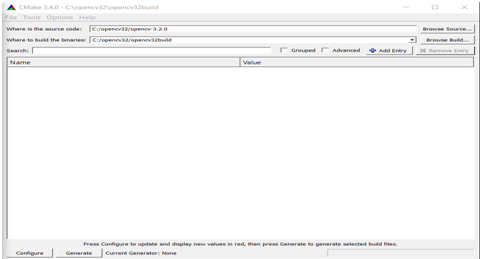
\includegraphics[width=0.9\textwidth]{img/working1.png}
\caption{ setting Cmake right directories }
\label{fig:working1}
\end{figure}

\item we can hit several times  configure. Until we have some list of possible settings like on image below. Use different settings and configuration options. choose  solution we want. FFMPEG, OPENCL support and \textbf{generate OPENCV.SLN file inside  opencv3.0 build folder.} 

\begin{figure}[H]
\centering
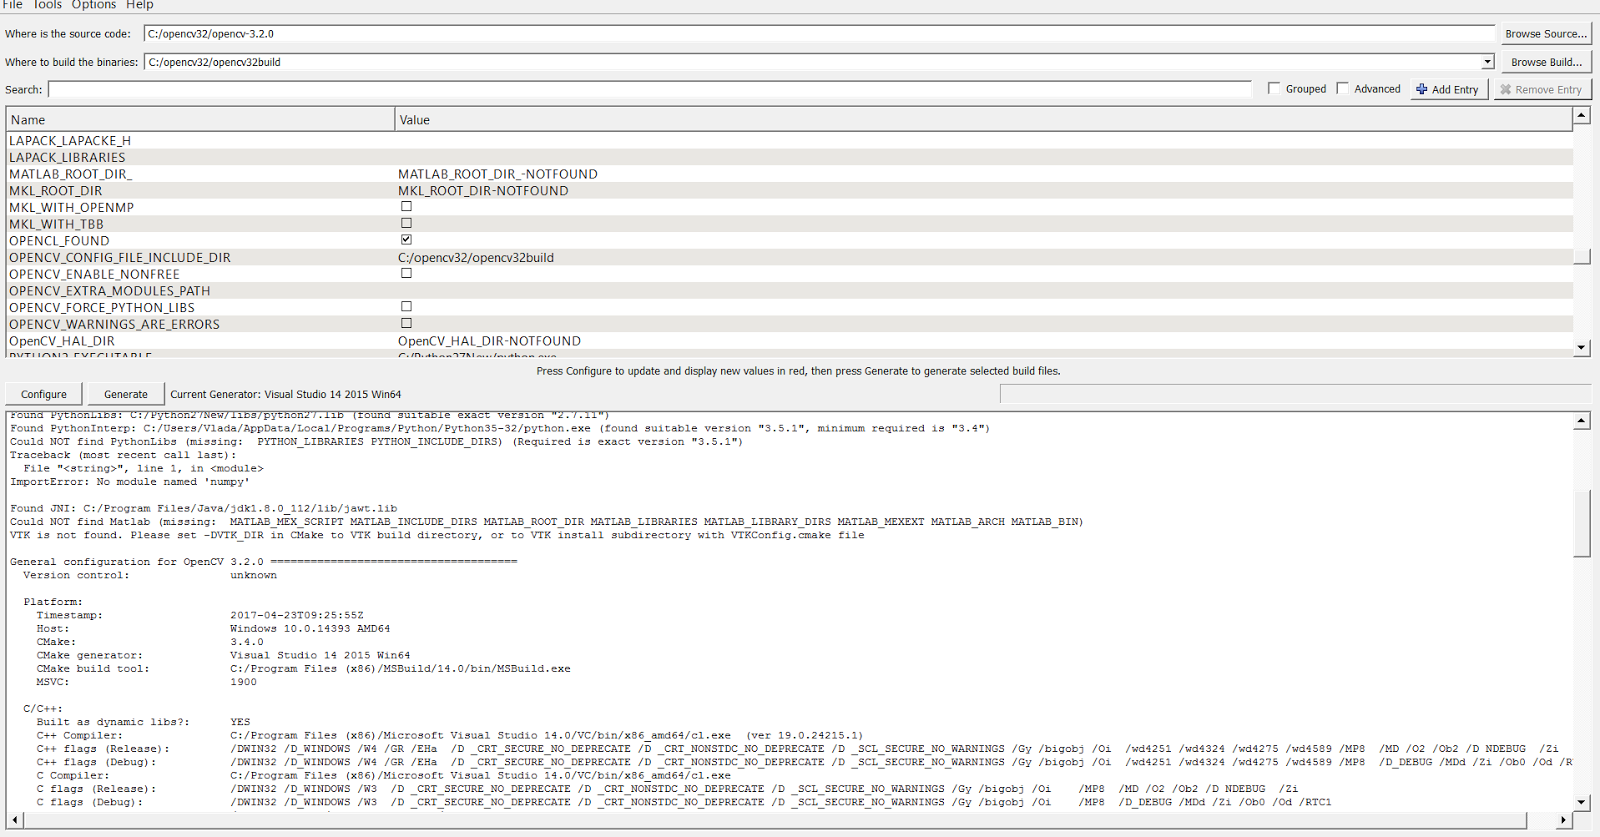
\includegraphics[width=0.9\textwidth]{img/working2.png}
\caption{ result after building }
\label{fig:working2}
\end{figure}

\item FIRST just select DEBUG, x64 version like on picture, click right mouse on Entire solution and hit BUILD the  solution should look like on the next figure . 
\begin{figure}[H]
\centering
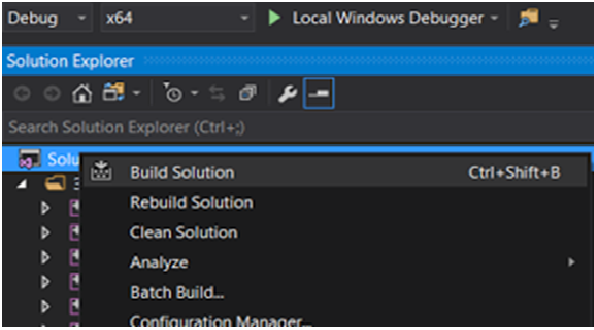
\includegraphics[width=0.6\textwidth]{img/working3.png}
\caption{ building solution}
\label{fig:working3}
\end{figure}

\item 	Second you need to switch from DEBUG to RELEASE and build the solution again. \textbf{This build} also Cmake target install, (you can see this under install) where  your installation is located. \\
Your installation location usually is under opencv32build/install .

\end{enumerate}

\subsection{linking Visual studio with opencv :}

\begin{enumerate}
\item OpenCV visual studio and create a console application 
\item in configuration Properties -$> C/C++ $-$>$ Additional Include Directories , then add OpenCV's Includes folders :
 \begin{itemize}
     \item C:/opencv/build/include
     \item C:/opencv/build/include/opencv
     \item C:/opencv/build/include/opencv2
   \end{itemize}
\item in configuration Properties -$>Linker$-$>$Additional Library Directories -$> $ add folder lib of OpenCV :\\
     C:/opencv/build/x64/vc14/lib 
\item in configuration Properties$->$ Linker$->$Additional Dependence$->$ add folder lib of OpenCV .
 \begin{itemize}
     \item opencv\_world320d.lib
     \item opencv\_features2d320d.lib
     \item opencv\_xfeatures2d320d.lib
   \end{itemize}

\end{enumerate}

